\chapter{Understanding data entry in an office setting}\label{ch:12}
\begin{mynote}
\subsubsection{Chapter outline}

This chapter reports an interview study on understanding data entry work in a naturalistic office setting, and a contextual inquiry study on how people self-interrupt in this setting. Participants try to avoid task-irrelevant interruptions, and postpone physical inquiries if they expect them to take a long time, but digital inquiries are addressed immediately. Together these studies suggest that people do not always know how to effectively manage self-interruptions if they are seen as part of the same activity, because of preconceptions about ease of access, and because of lack of awareness of time spent on digital interruptions.
%Together these studies show that participants have to look up information from sources with differing levels of time costs. Whereas for paper sources, time costs affect whether it is addressed now or later, they interrupt immediately to gather digital information. This suggests that people are unaware of the time spent on digital interruptions. 

\end{mynote}

\section{Introduction}
To address the aim of this thesis, which is to understand how people can better manage the time spent on inquiries needed for a data entry task, it is important to not only look at people's data entry performance using a well-structured task, but also at data entry in the environment in which these tasks are normally performed. \citet{Bondarenko2005} showed that the type of task influences how people manage information and therefore might impact how they address inquiries.\looseness=-1

The aim of the studies reported in this chapter was therefore to get a detailed understanding of data entry work in a finance office setting and how people currently manage inquiries for this type of work. In particular, the aim of Study \hyperref[st:Study1]{1} was to get a grounded understanding of data entry work, the physical environment, and the type of information sources needed for this type of work. Office workers were interviewed at their workplace about their data entry work and asked to demonstrate a typical data entry task. The aim of Study \hyperref[st:Study2]{2} was to understand the different time costs associated with information sources, and whether this affected people's self-interruption behaviour. %Study 1 revealed that a major aspect of data entry work in this setting is collecting information from multiple sources with different levels of access, which then became the focus of the rest of the thesis. The contextual interview study showed office workers regularly interrupt themselves as soon as they realise they need digital information, but barely interrupt themselves to access paper sources as there is effort involved. Digital interruptions took longer than intended as participants were distracted by task-irrelevant information.

\section{Study 1: Understanding data entry work in a financial office}\label{st:Study1}
 
\textit{This study was published in \citet{Borghouts2017} and presented at the European Conference on Computer-Supported Cooperative Work in 2017.}
 
\subsection{Introduction}
As data entry is a common task and it is important this is done both accurately and efficiently, work has been done to design and optimise data entry interfaces to support fast and accurate data entry \citep[e.g.][]{Oladimeji2013, Vertanen2015, Wiseman2013a}. Studies have shown that creating interfaces to slow down data entry \citep{Gould2016b}, by requiring additional information \citep{Wiseman2013a} or using alternative input technology \citep{Oladimeji2011} can all reduce error rates in the lab. However, these solutions do not always work outside of the lab \citep[e.g.][]{Gould2016b}, as it is not just the data entry interface that determines efficiency and accuracy but also other aspects of the task, such as the environment within which it is conducted \citep{Payne2013, Randall2014}. For instance, in lab studies, users are given clear instructions and are given the data to enter. 

In everyday computer use, data entry tasks might not be so clearly prescribed \citep{Evans2012}. To illustrate, \citet{Evans2012} investigated if people's data entry behaviour in a lab setting was comparable to how they would normally perform these inputting tasks in their everyday life. They remotely observed people's input behaviour on their personal computer, and compared this data with their performance on similar tasks in a lab. Participants installed a tool on their personal computer which logged all data entry and mouse pointing behaviour they performed in one work week. Examples of tasks that were carried out were sending personal messages to friends and browsing the web. There were no differences in uncorrected errors or data entry speed between the lab and the field, but they did find that participants corrected more errors in the lab. The study shows that people check and correct their entries more when they are in a controlled environment and are focused on the task, though the measured behaviour on people's personal computers mostly included tasks where accuracy may not have been considered important, such as sending an informal chat message to a friend. 

The aim of Study \hyperref[st:Study1]{1} was to get an understanding of people's data entry work in an office setting. As the nature of this first study was exploratory, semi-structured interviews were considered to be an appropriate method for this purpose. Participants were able to further explain their strategies and discuss challenges they experienced. Furthermore, it enabled the collection of participants' experience with past critical incidents, which may not be captured in observational sessions. The study explored people's data entry work overall, and the focus of this study was not specifically on people's information behaviour. As data collection and analysis progressed, information collection was found to be a large and integrated part of people's data entry work, which could potentially influence their performance. After this study, people's information behaviour became the focus of the next study.

The user group of this study were office workers at finance administration offices at two public universities, who conduct data entry tasks as part of their daily work. This user group was chosen as they have a lot of data entry tasks as part of their job, and it is an area where it is important to enter data accurately, but there is also time pressure to finish work on time. Furthermore, it was an accessible user group to approach.

\subsection{Method}
\subsubsection{Participants}
Nine participants (five female, four male) took part in the study. They were employees from two public universities and their work involved receiving various requests for payment, checking the information in these requests was correct, and entering the information along with administrative data into computer systems. Ages ranged from 18 to 52 (two participants wished to not disclose their age). Their level of experience in this type of job ranged from one to 17 years. All but one (P2) worked full-time. Table \ref{tbl:ch12-Table1} shows further demographic details of the participants. Typical data entry tasks participants dealt with were checking and entering expense forms sent by staff and students, paying salaries and pensions, controlling research budgets, monitoring university income and expenses and entering employee information. Participants were recruited by sending invitations to opt-in mailing lists of Finance departments, and were reimbursed with a \pounds10 Amazon voucher.

\begin{table}
\caption[Study 1 participant information]{Participant information.}
\centering
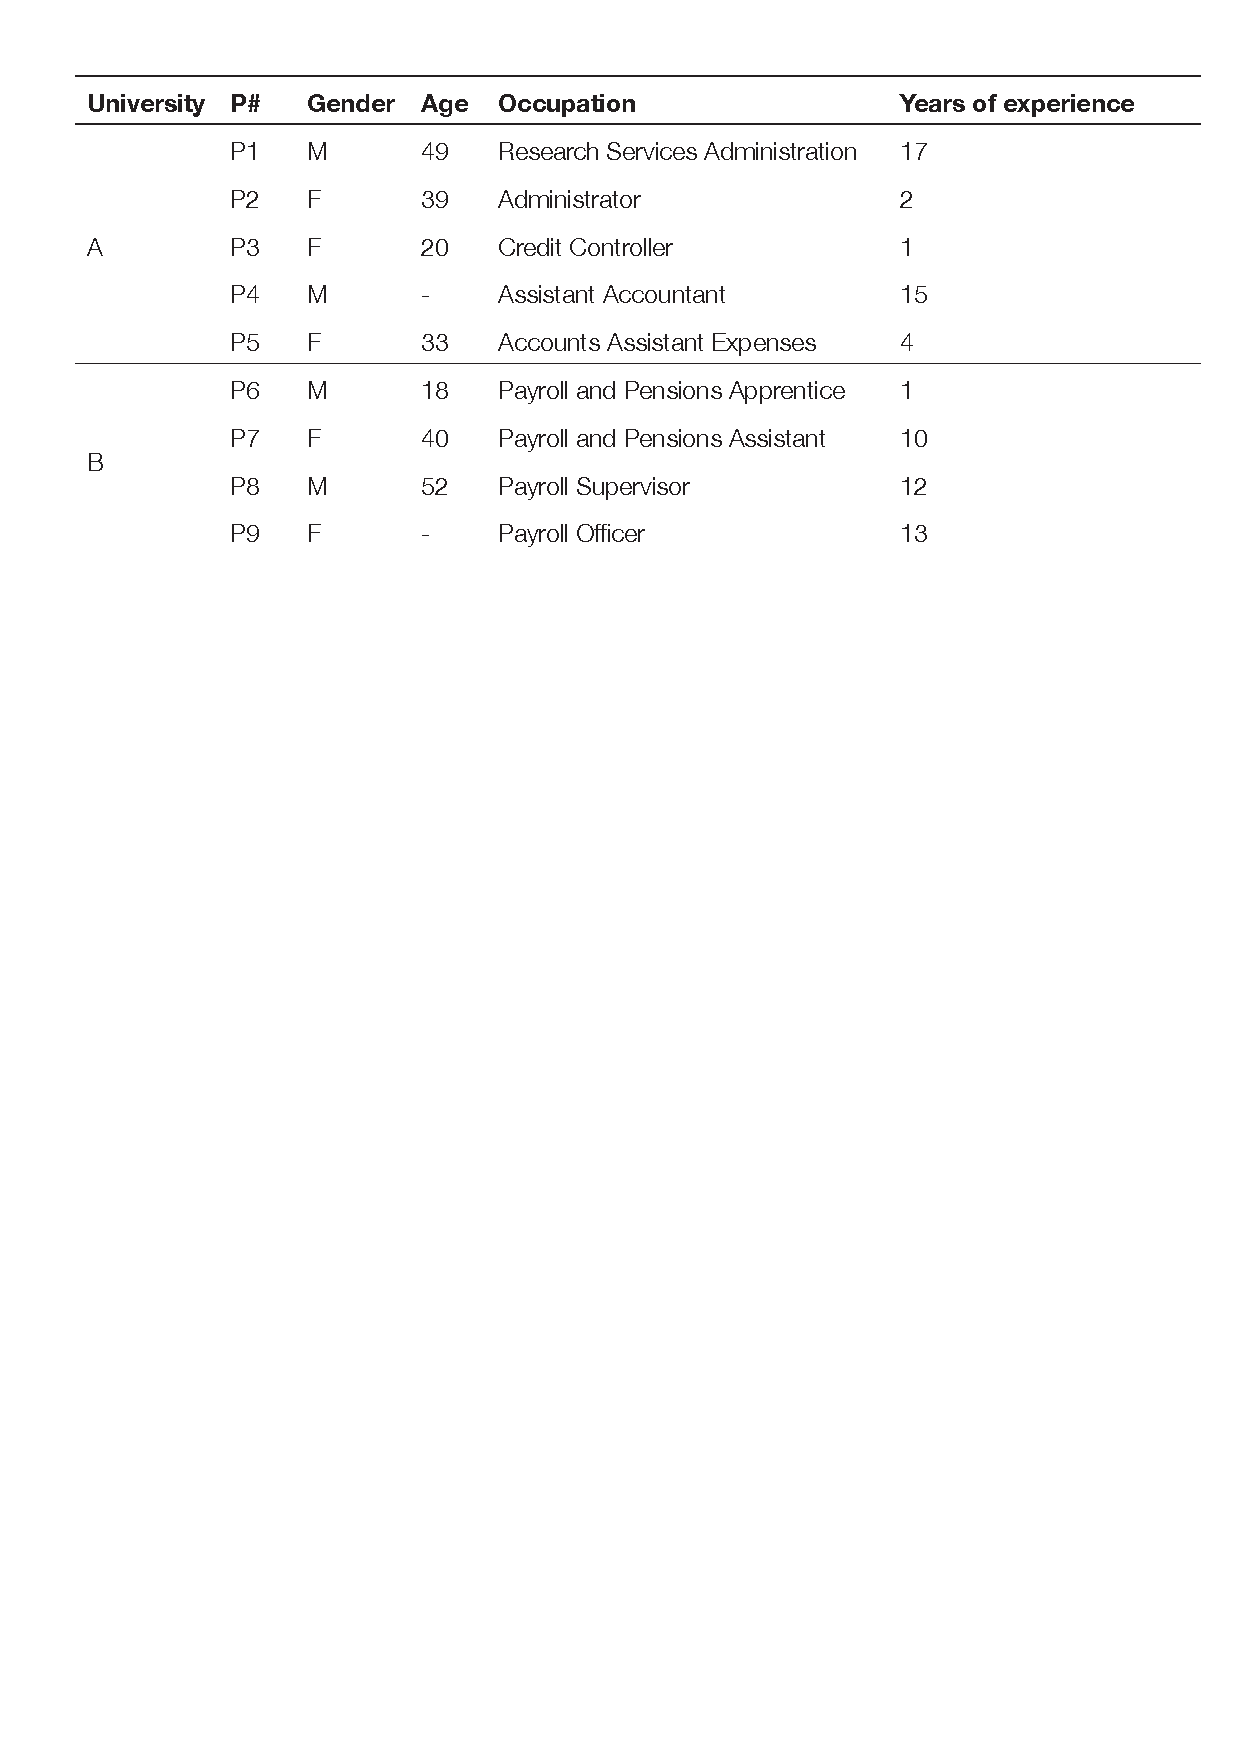
\includegraphics[width=0.9\textwidth]{images/ch12/ch12_participants.pdf}
\vspace{-3pt}
\label{tbl:ch12-Table1}
\end{table}

\subsubsection{Materials}
Materials that were used during the interview were a voice recorder, a paper copy of an interview script with the interview topics and guiding questions, a consent form, an information sheet for the participant and a notebook and pen to make notes. The interview script, information sheet and consent form are included in Appendix \ref{ch:S1_Materials}.
Each interview covered four guiding topics, which are briefly described in Table \ref{table:ch3_interviewtopics}. For each topic, a number of questions were written out beforehand. These questions were used as a starting point to get the participant talking and guide the interview. Based on what the participant was saying follow-up questions were asked. %The audio transcription program ExpressScribe was used to transcribe the interviews. The data analysis programs Nvivo and Atlas.ti were used to analyse the data. Nvivo was used to code the interview transcripts and notes. Atlas.ti was used to complement the analysis in Nvivo and allowed to identify relations between codes.

\begin{table}[htp]
\centering
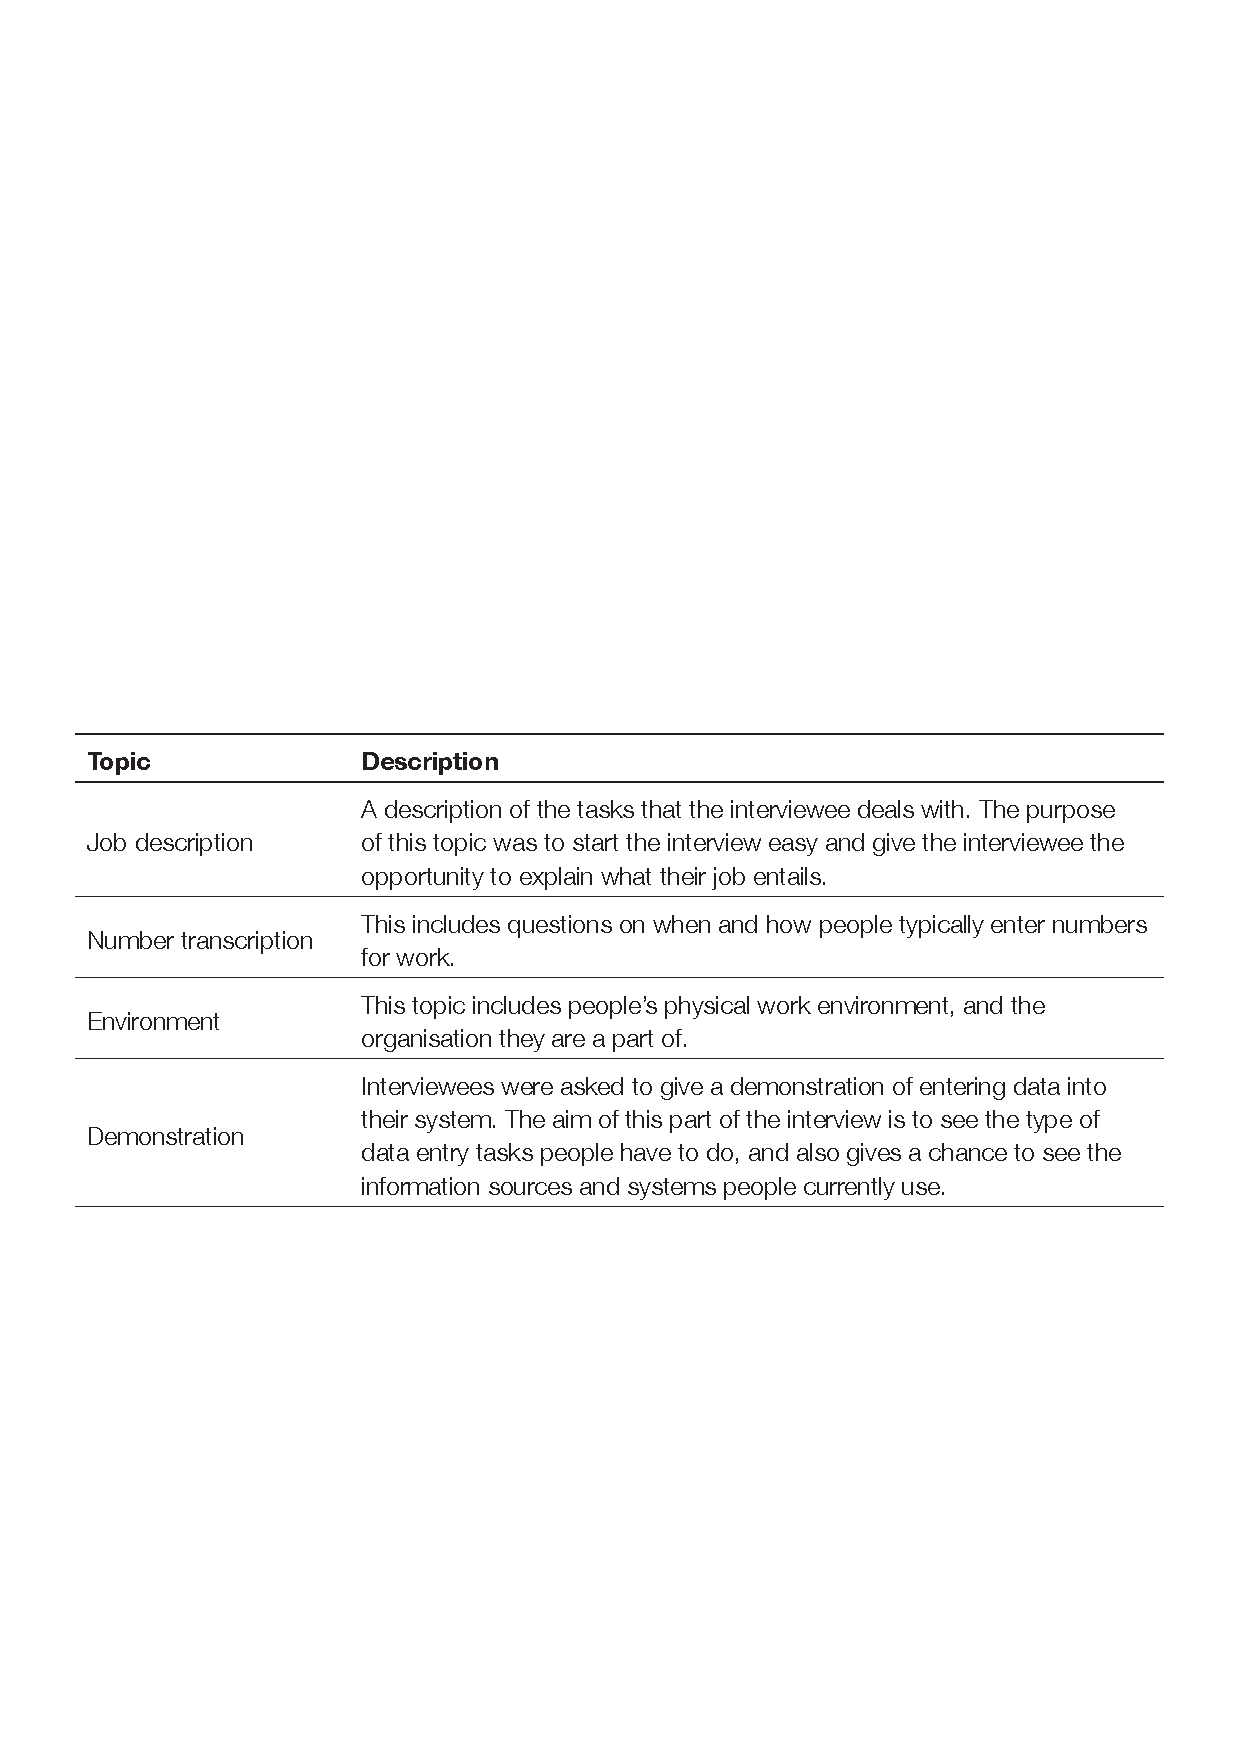
\includegraphics[width=\textwidth]{images/ch12/ch12-1_InterviewTopics.pdf}
    \caption[Study 1 interview topics]{Interview topics to guide the interview.}
    \label{table:ch3_interviewtopics}
\end{table}%

\subsubsection{Data recording}
A voice recorder was used to audio record the interviews. One participant wished to not be audio recorded and one interview could not be audio recorded due to technical issues, so for these two interviews notes were taken of the answers. For the remaining seven interviews, notes were only made of observations and not the participants' answers. Notes were made with pen and paper. Photographs were made of the work environment and screenshots of the systems that the interviewees used.

\subsubsection{Interviewing procedure}
The interviews took place at the participants' workplace. For two interviews, the interviewee's office place was not suitable for talking so the interview took place in a common room nearby, and these participants showed their workplace and completed a demonstration of entering data after the interview. Participants were welcomed and informed about the study. They received a paper information sheet with the outline of the study and contact details of the researcher to keep for future reference. They were also asked to read and sign a consent form. They were asked permission for the interview to be audio recorded, and could still participate if they did not wish not to be audio recorded. 

%Participants were informed that the data would be used for research purposes only and stored in accordance with the Data Protection Act 1998. They were also informed that their data would be anonymised and when used in a report or academic paper, their data would not be directly identifiable. Names of participants or the universities they were working at were not included in the interview notes and transcripts.

The interviews were semi-structured and took between 20 and 55 minutes. Each interview was reviewed afterwards, and findings sometimes fed into new questions being included or some questions being adapted in subsequent interviews.

\subsubsection{Pilot interview}
A pilot interview was conducted with an acquaintance of the researcher who worked in Finance, to test out the set-up of the study and questions. The interview took place at the participant's home, notes were taken with pen and paper, and the interview was audio-recorded using iMovie on a Macbook Pro. 

Taking notes slowed down the flow of the interview: sometimes the interviewee stopped talking to give the interviewer the opportunity to finish taking notes. Furthermore, taking notes took attention away from what the interviewee was explaining: assumptions made during the interview did not seem to be accurate in later analysis. Therefore, it was decided that note taking would be kept to a minimum. Notes would only be made of observations that could not be taken from audio recordings.

%The interviewee talked elaborately about manually converting different currencies, and identified this task as the main place where errors occurred. Therefore, questions were included about if interviewees dealt with foreign currencies and converting these. 

\subsubsection{Research Ethics}
All studies in this thesis were undertaken with ethical approval from the UCL Research Ethics Committee [Project ID Number UCLIC/1415/001/Staff Brumby/Borghouts]. Study participants were informed what would happen to their data, and data was handled in accordance with the Data Protection Act 1998. Participants were informed that their data would be anonymised and when used in a report or academic paper, their data would not be directly identifiable. Names of participants or the universities they were working at were not included in the interview notes and transcripts. Information sheets and consent forms provided to participants followed UCL guidelines, and are included in the Appendix. 

\begin{comment}
\subsubsection{Ethical considerations}
The study was undertaken with ethical approval from the UCL Research Ethics Committee [Project ID Number UCLIC/1415/001/Staff Brumby/Borghouts]. 
At the start of each interview, participants were first informed verbally about the study. They were then given a consent form to read and sign, and were given an information sheet to keep. This information sheet contained the study information and contact details of the researcher and the project's principal researcher, should participants have any further questions after completion of the study.  They were asked permission for the interview to be audio recorded. One participant wished not to be audio recorded and notes were taken instead. 

Participants were informed that the data would be used for research purposes only and stored in accordance with the Data Protection Act 1998. They were also informed that their data would be anonymised and when used in a report or academic paper, their data would not be directly identifiable. Names of participants or the universities they were working at were not included in the interview notes and transcripts.
\end{comment}

\subsection{Results}
\subsubsection{Data analysis}
After each interview or set of interviews, a first analysis took place. The audio recording was played back, notes were typed into a digital file and reviewed and the interview was transcribed verbatim. Several non-verbal cues were included in the transcripts as well, such as when the interviewee laughed or sighed, as well as descriptions of when the interviewee was demonstrating something. The advantage of doing the transcription shortly after the interview was that it was still easy to remember from listening to the audio recording what was being demonstrated. Interesting findings and initial patterns that were apparent across the data were written down. 

After all interviews had been transcribed, the transcriptions and notes were printed and the data was analysed using thematic analysis \citep{Braun2006}. An inductive approach of thematic analysis was used: there was no pre-existing coding scheme, and codes were created based on what emerged from reading over the transcripts and notes. Anything in the data that was considered to be interesting was annotated by hand and labelled with an appropriate code. On reviewing the coding, some codes were grouped together in one code, additional codes were named, and similar codes were grouped under themes. For instance, an initial code was Notifications, such as e-mail notifications. During the second coding iteration, it was identified that people always talked about notifications in the context that they were interrupted (by a notification) rather than about notifications on its own. Therefore, notifications and interruptions were grouped into one code. 

The codes were then reviewed, to see if they addressed the purpose of the study. The transcripts and notes were then imported into Nvivo and Atlas.ti and coded digitally. Nvivo was used to get insight into the occurrence of codes. Atlas.ti was used to complement the analysis in Nvivo, and allowed the identification of relations between codes.

%The transcripts and notes were then imported into Nvivo and coded digitally. Atlas.ti was used to complement this analysis and allowed to identify relations between codes. 

%The audio transcription program ExpressScribe was used to transcribe the interviews. The data analysis programs Nvivo and Atlas.ti were used to analyse the data. Nvivo was used to code the interview transcripts and notes. Atlas.ti was used to complement the analysis in Nvivo and allowed to identify relations between codes.

\subsubsection{Themes}
In total 51 codes were derived, and these were grouped into 8 main themes, which are listed and described in Table \ref{table:ch3_themes}. If codes or separate quotes did not belong in a certain theme but were still considered relevant, they were grouped in the Other category. 

\begin{table}[htp]
\centering
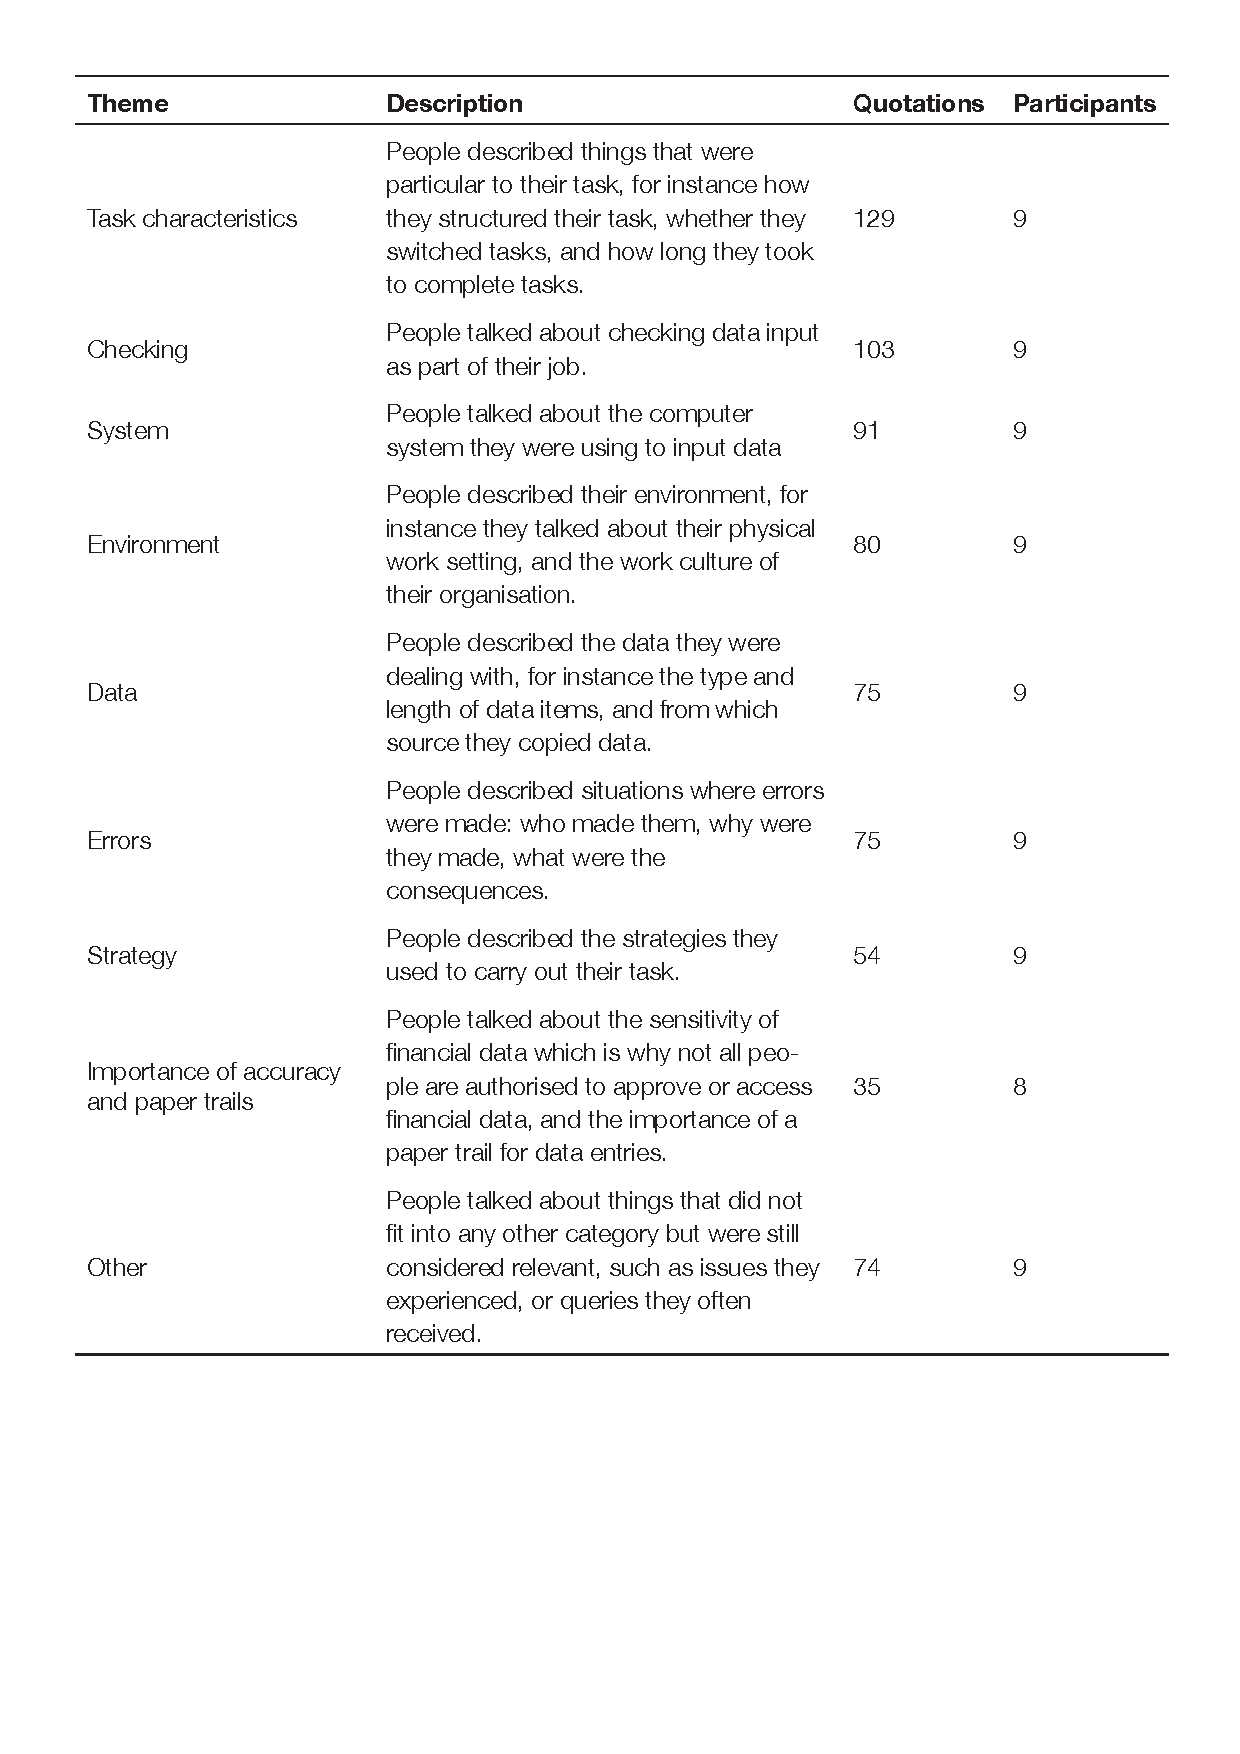
\includegraphics[width=\textwidth]{images/ch12/ch12-1_Themes.pdf}
    \caption[Study 1 interview themes]{The themes that emerged from the interview data, along with a description. The column Quotations indicates how many times this theme was brought up during interviews, and the column Participants indicates how many participants talked about it.}
    \label{table:ch3_themes}
\end{table}

Themes were visualised as diagrams, which are included in Appendix \ref{ch:S1_Diagrams}. Each diagram shows a theme's main codes and relationships between codes, the number of quotes that were grouped under this theme, and the number of interviewees who mentioned it. These diagrams helped to gain insight how codes were connected, and also how prevalent topics were across the collected data. 

In the following Results section, I report the key findings from the analysis.  The diagrams are included in Appendix \ref{ch:S1_Diagrams} to make transparent how data was analysed and to clarify what I base the key findings and conclusions on. I first describe the data entry work participants dealt with, to provide context to the type of work I focus on in this thesis. I then discuss how people scheduled their work, the information sources they dealt with, and current strategies people described to improve data entry performance.

\subsubsection{Type of data entry tasks}
A common data entry task was processing expenses. Participants received requests from university staff and students, who had spent money for research purposes and wanted to claim back the expenses. Participants had to check the information they were given was correct. For instance, they had to check that the amount being claimed back matched the value on the original receipts, and that the expense fell within permitted limits. In addition to transcribing and checking individual numbers, participants also mentioned they often have to perform and check calculations, for example to check that all individual expenses were converted correctly from a foreign currency. After checking the data and calculations, they then had to enter the data, along with other information such as budgeting and staff information, into a computer system. The time spent on processing a single expense claim differed: checking data on a short expenses form could be completed in two minutes, while a single manual calculation could take between 20 and 30 minutes. Two participants described dealing with a lot of data entry as time-consuming and tiresome.

Participants primarily dealt with numeric data, such as financial data and IDs. The monetary numbers they dealt with ranged from five pounds to millions of pounds. Participants also entered and checked alphanumeric and non-numeric data such as employee names, addresses and bank account details. Numeric data consisted of individual numbers, as well as groups of numbers that together made up a new number, such as the total amount of money spent on a project. Participants had to both check and transcribe each individual number, and check that the calculation was correct. 

\subsubsection{Scheduling data entry work}
The workload varied throughout the year. Four participants mentioned that their work followed a work cycle and they did different things at different times of the month. One week could be reserved for checking all the data they received from another department, while another week could be spent on solely inputting data. Participants reported that they dealt with between 30 and 80 expense claims per day. The amount of individual data items to enter averaged to 6,000 items a day. 

To complete data entry work efficiently, eight participants saved up data entry tasks, to enter all data in one sequence. If they received new data entry tasks, they often did not work on them immediately, but instead waited until they had several saved up and then completed all of them in a single batch. P2 was the only interviewee that processed forms with numbers to enter as they came in. She only dealt with a couple of claims per day, and did admit that if she had more data to fill in, she would probably do it in a more efficient way.

The reason participants gave for batching data entry work was that they found it quicker and easier to do the same type of task in one sequence, before they started another type of task. Participants did not have specific deadlines set by their organisation to finish certain expenses. Some said they saved them up but did try to finish expenses before the next payroll was due, so that claimants could get their expenses reimbursed on time. P6 explained he postponed processing expense forms until the deadline to submit forms for that month has passed, after which he did all forms in one sequence: \textit{"When I’m doing it lots at a time, I think once you get into sort of the hang of it, it gets done a lot quicker."} (P6)

\subsubsection{Interruptions}
Participants batched data entry work, and tried to concentrate on the task at hand, and avoid self-interruptions to other tasks: \textit{"I try to concentrate on my task...I try to do one task (i.e. doing all expenses), finish one, and then do another."} (P9). All participants did attend to some external interruptions, which they considered part of their job: P8 had to pause his task immediately if a staff member entered his office and needed his help. Other participants mentioned they primarily tried to concentrate on the task at hand, but did briefly glance over e-mail notifications, to see whether something important needed their attention.

\subsubsection{Information sources}
While participants avoided task-irrelevant interruptions during a data entry task, they did have to interrupt and leave the data entry system to look up information related to the task and then return to the system window to enter it. The information needed for one task was usually spread over several windows on the computer, so participants had to flick back and forth or memorise certain information from one window to use in another window: \textit{"Depending on the input, it can be quite complicated, and there are quite a lot of different screens to input."} (P7). All participants had their computer windows maximised, so one window covered the whole screen and participants could not look at the data entry window and information source concurrently. Participants said that if they had to get out of the system to look up information digitally and then get back to the system window to enter it, they preferred to memorise the information, rather than flick back and forth and look it up each time they needed it: \textit{"I wouldn't necessarily have to [memorise it], it's more (…) if you have to keep flicking back to different things, it's sometimes just easier to try and remember it. But you can obviously take the long version and keep flicking back to the correct screen."} (P3). Data items that had to be entered frequently such as project codes, were memorised even if participants did not deliberately choose to do so.

The data was spread across both digital and paper sources, and participants had to switch between computer windows and physical locations to retrieve all data required for a single expense claim. Examples of digital sources were spreadsheets, text documents, departmental databases and e-mails. Examples of paper sources were receipts, claim forms, and print-outs of spreadsheets. Participants worked with paper sources for two main reasons. First, digital information was printed out to keep it nearby. P7 and P8 had printed out information they frequently needed to look up and had placed this nearby on their desk, so they could easily use this to check if the input they had received was correct. Second, some documents had to be in paper form for auditing purposes, because participants were working with sensitive financial data. Hard copies of receipts and signed paper claim forms had to be archived and were checked by external auditors. People also explained they liked to write out and keep a record of manual calculations, in case someone had any questions on how figures was calculated.

\subsubsection{Checking for data entry errors}
Even though participants discussed that they tried to focus on data entry tasks by avoiding task switches, they did discuss that data entry errors still happened frequently. Errors that were made were typos, miscalculations, or the wrong information altogether. The main explanation people gave for errors was that it is human to make mistakes, but it was also mentioned people are under time pressure, and that people rely on the fact it will be checked by another person, which makes them less careful in entering accurate data. P9 attributed it to having to switch between computer windows. P4 attributed errors to the use of both paper and digital files: he felt it was much easier to make an error and omit figures when transcribing from paper sources.

Errors had negative consequences on people's work. If an error was spotted and was sufficiently small, it could be processed or corrected without negotiation, but if it was a large error, it had to be sent back or forwarded to a higher authority for approval. This considerably slowed the process down. Furthermore, P8 warned that even with extra human checks not all errors get caught, which meant errors could be made with paying back claimants.

The main method to prevent errors was to have data input visually checked by multiple people before it was processed for payment. People's experience with this checking system differed: P3, a credit controller who was one of the first people on her team to enter the data before it went to another colleague, believed it increased the chances of an error being caught because it goes through so many different checks. In contrast, P8 and P9 argued this made people even less careful about making errors. As payroll supervisors, they were the last persons at their office to check data before it was submitted to the system and processed for payment. They commented that even at this last stage it was still quite common to spot data entry errors: \textit{"The departments actually sometimes treat us as a checking system [laughs], but they shouldn't really. (…) even though we are like a second check, we feel sometimes that we are the first checkpoint."} (P9).

\subsection{Discussion}
The aim of Study \hyperref[st:Study1]{1} was to gain a better understanding of data entry work in offices, and the physical environment in which these are conducted. For this purpose nine interviews were conducted with office workers from two public universities who worked with financial data. The main findings of the study are: 

%The purpose of this study was to gain a better understanding of data entry work in financial offices, and the physical environment in which these are conducted. For this purpose nine interviews were conducted with office workers from two public universities who worked with financial data. 

\begin{itemize}

\item 
data entry work is batched, so people can enter a lot of data entry at once, and minimise interruptions to other tasks. 
\item 
data entry tasks have to be interrupted to retrieve data from multiple information sources
\item 
data entry errors are common, and the current solution is to have data entered and checked by multiple people before it gets submitted to the system
\end{itemize}

In the next sections, I first compare the findings with prior research, before concluding what we learn from this study. 

\subsubsection{Batching data entry work}
Though participants received data entry tasks on an ad-hoc basis, most of them saved them until a specific moment and then processed them all in bulk. People stated that it made them faster in entering data, and they preferred to focus on one type of task at once. Prior experiments have shown that people do become faster in data entry over time, but also more erroneous \citep{Healy2004}. Data entry interfaces that slow people down have been shown to reduce errors \citep[e.g.][]{Gould2016b, Oladimeji2011}, but these studies tested up to 240 number entries, whereas participants in the current study reported they often had to enter around 6,000 numbers a day. Interfaces that slow people down may therefore not be applicable in the setting of the current study. \citet{Healy2004} recommend regular breaks when entering large amounts of data to maintain accuracy. However as participants in this study were free to schedule their data entry work and deliberately chose to schedule all their data entry in one session, it may be challenging to initiate and take work breaks. 

\subsubsection{Fragmentation of work}
Contrary to prior data entry research, information was not located on one source but was scattered across physical and digital information sources. Furthermore, in data entry experiments people are often only presented with the data they have to enter and sometimes are given only one data item at a time. The sources from which people had to enter data in this study usually contained a lot of data, not all of which was relevant to the task: sometimes participants had to go through a large spreadsheet, before they found the number they needed to copy. The amount of irrelevant data on the sources can increase the time people need to look up the information they need. 

This fragmentation of work is consistent with prior workplace studies that found  office work often involves switching between different sources \citep{Cangiano2009, Czerwinski2004, Mark2005, Sellberg2014}. In the current study, the time cost to access these information sources also differed. For instance, some paper sheets were on people's desk, but some paper sheets had to be retrieved elsewhere. Participants also dealt with multiple windows on their computer screen, and sometimes needed to switch between different windows. Instead of flicking back and forth to view information they had to enter in another window, participants said they preferred to memorise it, even though they could also write the information down or in some cases copy and paste it, which would be a more accurate strategy. This behaviour can be explained by the soft constraints hypothesis, which states that people increasingly rely on information in memory, as more effort is involved in cognitive offloading or accessing external resources \citep{Gray2006}. This strategy allows people to be faster, but carries the risk that they misremember information. In previous studies, trying to hold more items in memory during a copying task increased errors \citep[e.g.][]{Borghouts2015, Morgan2009}. However, in these studies participants had to copy unfamiliar data. In the current setting, the information had some meaning to users and some items were entered more often than others. These familiar numbers are more strongly represented in memory \citep{Wiseman2014}, in which case a memory-based strategy may be less error prone.

The understanding that entering data is only one part of the broader data entry task flow can inform future data entry research and improve the way data entry tasks are modelled in lab-based experiments. In most data entry experiments, data is given and presented to the user in an organised manner. Future lab-based studies could require participants to first collect data from multiple sources, in order to see how it affects data entry performance. Having an experimental task that is more closely modelled to a situated task will give a better understanding to what extent different interventions are applicable. For example, slowing people down in data entry has shown to reduce errors in the lab \citep{Gould2016, Wiseman2013a}, but this intervention may not desirable if people are holding items in memory, or entering large volumes of data.

\subsubsection{Error checking}
Fragmented attention has been shown to have a negative effect on work performance \citep{Bailey2001, Carrier2015}, and participants in the current study reported errors happened regularly. To detect these errors, data input was visually checked by multiple people. This checking method resembles what \citet{Reason1990} describes as the Swiss Cheese model, where multiple checking layers are used to minimise the risk of errors. However, prior research has shown this is a poor checking method to check for errors in data entry \citep{Olsen2008, Wiseman2013a}. Despite being widely applied in practice, there is no strong support for the effectiveness of double-checking \citep{Li2016}. One of the reasons people may not detect errors when checking a colleague's entries is confirmation bias, which occurs when people selectively attend to stimuli that confirm one's belief \citep{Lewis1986}. People may expect data entries to be correct: participants reported they regularly received erroneous data, which had previously been checked and approved by several people. 

%\subsubsection{Limitations}
%An inductive approach was taken to analyse the data. However, it should be acknowledged that no researcher approaches research data completely neutral \citep{Blandford2013b}: data analysis was informed by pre-existing knowledge of data entry literature, which partially shaped the direction of the data analysis. Furthermore, interviews were semi-structured and follow-up questions were asked based on answers of the participant. 

\subsubsection{Summary}
The aim of Study \hyperref[st:Study1]{1}  was to get a grounded understanding of people's data entry work in an office setting. Through interviews with data entry workers, I found that a substantial part of this type of work is not just entering the data but also collecting it from multiple sources in the physical and digital work environment. This has often been overlooked in previous data entry work, and may have an impact on data entry performance. We also learn that data entry workers treat irrelevant and relevant self-interruptions differently: interview findings suggest that they try to work efficiently and avoid task-irrelevant interruptions during data entry work. People try to batch similar data entry tasks to avoid task switches, but then have to interrupt for the task to collect information sources, which are spread across the task environment with different time costs to access them. 

The study relied on people's own explanations of their practices. This gave insight into reasons why people may employ certain strategies, and through this method I was able to discuss critical incidents which would be unlikely to be uncovered through observation alone. A limitation of relying on people's self-reporting however is that they may not do what they say they do \citep[e.g.][]{Randall2014}. Though people gave short demonstrations to support their explanations, they were not shadowed doing their work for longer periods of time. Importantly, while we know that information is scattered across the environment, it remains unclear from these interviews alone how people go about accessing these - in other words, how do they manage inquiries with different time costs? Study 2 was therefore conducted to observe and understand how participants currently address inquiries for data entry work.

%Sometimes the cost to access an information source was low, and people could easily access it and look at it while entering it. Other times the cost was high, and people had to go back and forth between the window that showed the information, and the window in which they had to enter the information. Theory suggests that these different access costs have an impact on strategy, speed and accuracy. In previous experimental studies, an increase in IAC made people check the information source less and instead enter what was in their head. This can make people more efficient as it minimises switching between the information source and the input interface, but if the information in the head is wrong, it increases errors. In these previous studies, it increased errors, but the studies made use of abstract artificial information, which may have been too hard for participants to memorise. 
%In the current study, people had to copy numbers and text. Previous studies showed that when looking at text and/or numbers, a deeper encoding of the information in memory makes people more accurate in entering the information. 
%The next study aims to see if the effect of IAC on a copying task extends to copying numbers, which people have experience with copying and can more easily memorise.

\newpage

\section{Study 2: Managing inquiries for data entry}\label{st:Study2}

\textit{This study and its results are included in \citet{Borghouts2018} which is currently under review as a journal paper.}

\subsection{Introduction}
Study \hyperref[st:Study1]{1}  revealed that a substantial part of data entry work involved collecting required information from paper and digital sources before it could be entered into a computing system. The time and effort it took to locate different kinds of information sources varied: paper sources could be nearby on people's desks or situated further in another physical location, and digital information could be one click away, or people had to switch between multiple documents before they found what they were looking for. What was difficult to gather from interviews was how variability in the sources of information involved, and the time cost of locating them, affected how people decide whether to attend to, or defer, self-interruptions. Gaining an understanding of these interruptions is important to understand,  to inform the design of any interruption management tools aimed to reduce the disruptiveness of inquiries.

%because different strategies impact task performance

The aim of Study \hyperref[st:Study2]{2} was to investigate how participants self-interrupt to access information sources for data entry work. Based on previous literature examining the influence of information access costs \citep[e.g.][]{Gray2006}, it is hypothesised that participants will make fewer interruptions to information sources if these are harder to access. 

The aim of Study \hyperref[st:Study2]{2} was therefore to observe and understand how participants self-interrupt to access information sources for data entry work. A contextual inquiry was conducted with nine office workers from a similar population as in Study 1. In Study 2, the specific focus was on people's inquiry strategies. Participants were observed at their workplace, and asked to first carry out a data entry task while thinking out loud. Next, they were observed while they continued working as they would normally. As processing expense claims was a prevalent data entry task across all participants in Study \hyperref[st:Study1]{1}, I focused on this task.

Participants in the current study were video recorded while doing their expenses work. The video recordings captured the participants' interactions with the artefacts involved in the task, but the financial data on the information sources could not be identified from these recordings. The video recordings were used to supplement written observation notes, and after the observation part of the study, some video segments were played back to participants to explain what they were doing at certain moments.

\begin{comment}
The following questions were addressed in this study:

\begin{enumerate}
\item 
What is the information needed for an expenses task?
\item 
Where is this information retrieved from?
\item 
What are the strategies people use to look up information?
\end{enumerate}
\end{comment}

\subsection{Method}
My data collection was informed by using the methodological approach of contextual inquiry. Contextual inquiry is a combination of observation and interviewing users about their everyday work, with the aim to use the findings to inform design of the systems they use \citep{Holtzblatt2014}.
\citet{Holtzblatt2014} argue that observing participants carrying out their work can reveal concrete details, and it can help participants to recall past situations of carrying out work. It was therefore an appropriate method for the aim of this thesis, to understand how people can be better supported in managing inquiries for a routine data entry task.

\subsubsection{Participants}
Nine participants (four female, five male) took part in the study. Ages ranged from 27 to 52; three participants wished not to disclose their age. Participants from Study \hyperref[st:Study1]{1} were invited to participate again, but only one participant was able to participate again in the current study (P8 in Study 1, P1 in Study 2).  For the remainder of recruitment, a parallel sampling approach was taken \citep{Onwuegbuzie2008}. This approach means participants were drawn from the same population using the same recruitment techniques, but were not the same individuals. As in Study \hyperref[st:Study1]{1}, they were employees from financial offices at public universities dealing with processing expense claims. Table \ref{tbl:ch12-part2} shows further demographic details of participants. Participants had roles such as payroll officer, personal assistant, research manager, and administrator. Their experience in their current role ranged from one to 20 years. Participants were recruited through a combination of convenience and snowball sampling. They were invited to participate via emails sent to opt-in mailing lists of Finance departments, and emails forwarded by contact persons and people who had already participated.  

\begin{table}
\caption[Study 2 participant information]{Participant information.}
\centering
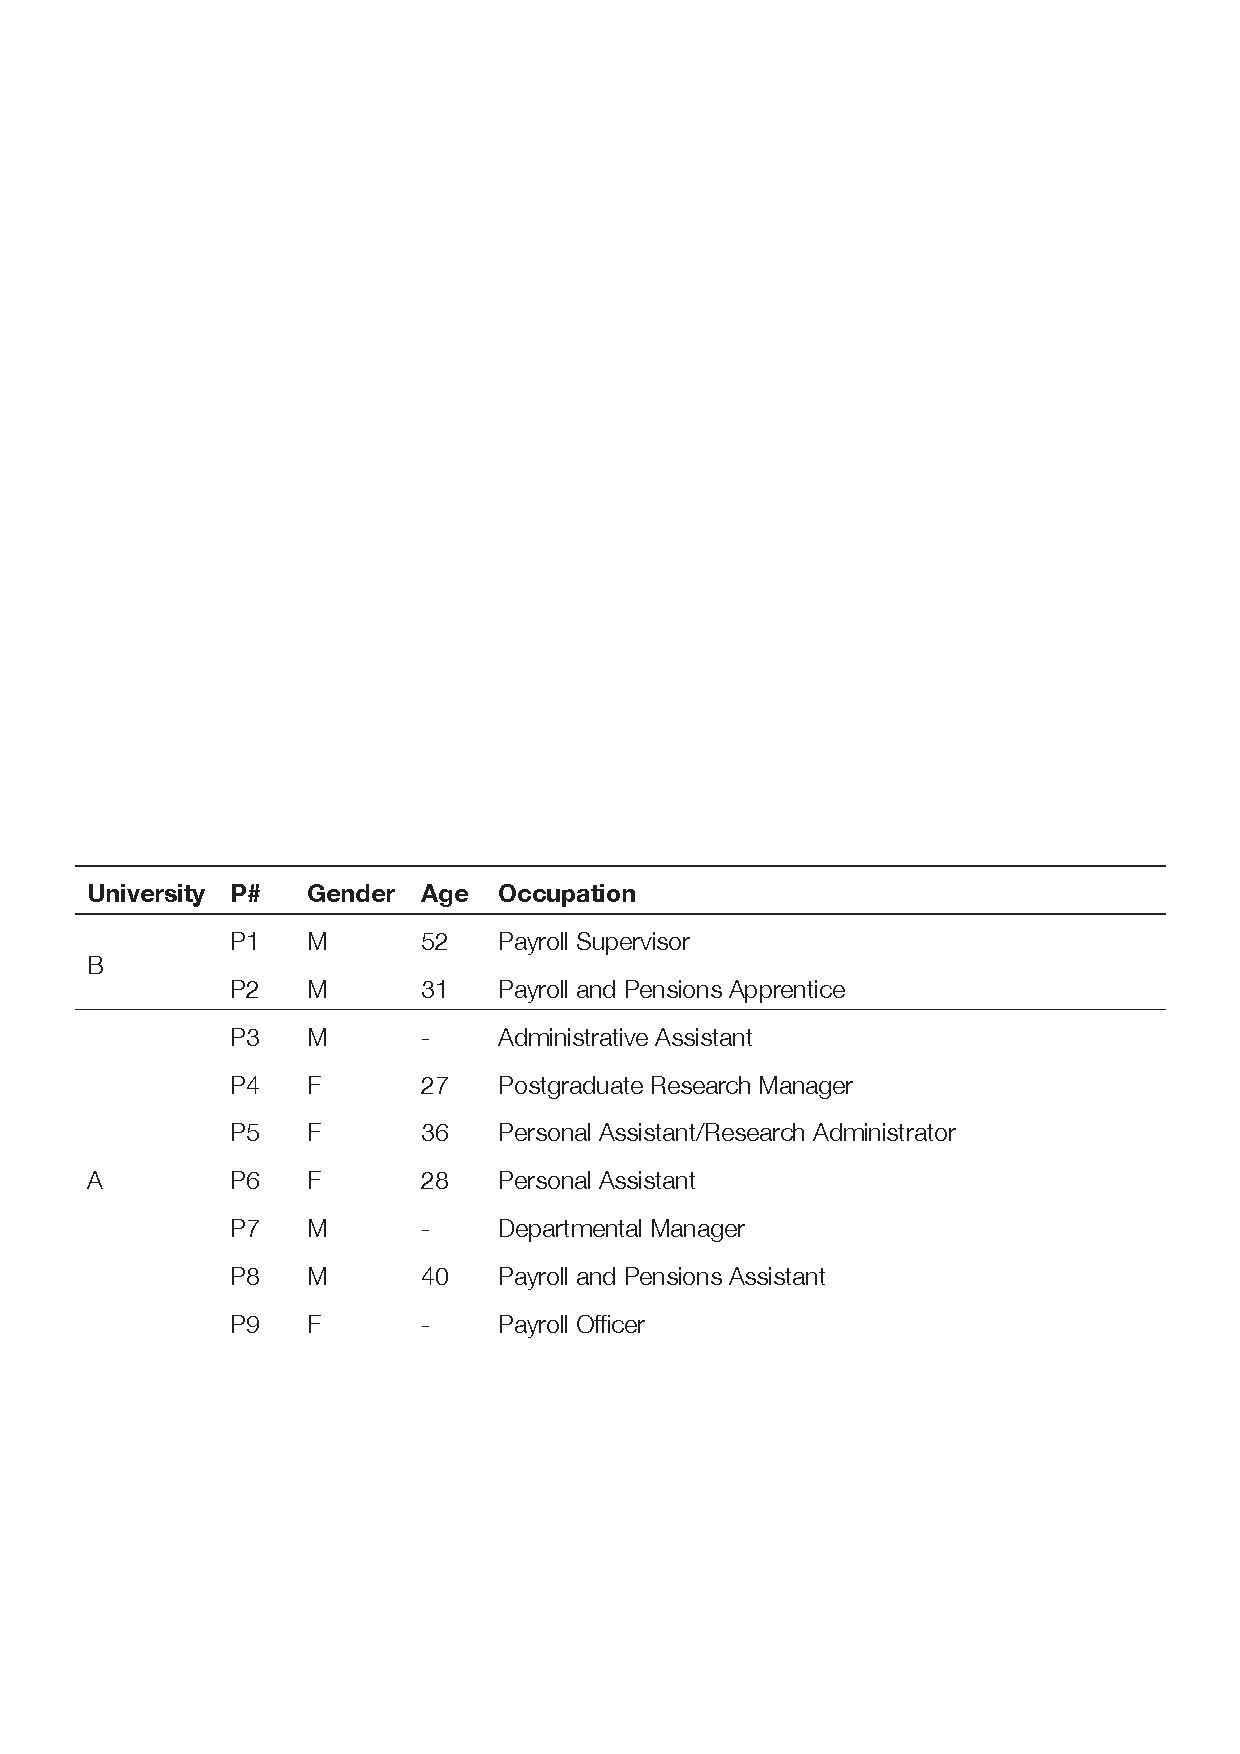
\includegraphics[width=0.9\textwidth]{images/ch12/ch12_participants2.pdf}
\vspace{-3pt}
\label{tbl:ch12-part2}
\end{table}

\subsubsection{Study setting}
The study took place in the same type of office setting as in Study 1. Participants were recruited from the same two public universities, and one office from Study 1 was visited again in this study. The other participants were from three different offices within these universities. They worked in open plan offices with two or more colleagues working nearby. 

\subsubsection{Procedure}
A single session with a participant lasted approximately 2 to 2.5 hours, and participants were reimbursed \pounds 15 for their participation. All sessions were audio and video recorded. The study protocol and interview script is included in Appendix \ref{ch:S2_Protocol}. A session followed four stages:

\begin{enumerate}
\item 
\textit{Interview.} Participants were briefed about the study and asked questions about the type of tasks they are involved in and the type of information sources they used. The aim of this interview was to make the participant feel comfortable and become familiar with the study, and for me to get an understanding of the participant’s work and job role. Participants were specifically asked about information sources they used.
\item 
\textit{Think-aloud.}  At this stage, the participant demonstrated processing an expense claim while thinking out loud. The participant was asked to elaborate if something interesting or unusual happened, or if the participant fell quiet.
\item 
\textit{Observation.}
After demonstrating the task out loud, the participant continued to process expense claims as he/she would normally without explaining what he/she was doing, while I observed and took notes.
\item 
\textit{Summary.} The session ended with a short interview and debriefing session. I summarised findings and confirmed with the participant if these assumptions were correct. If some parts of the observation needed clarification, segments of the video recording were played back to the participant, and he/she was asked to explain what was happening during these moments.
\end{enumerate}

\subsubsection{Pilot study}
Initially, the intended method for this study was to conduct a contextual inquiry, followed by a week-long diary study where office workers would log diary entries of their expenses tasks. The aim of this diary study would be to get a further insight in additional information sources the workers may sometimes use, that were not covered in the contextual inquiry.  Participants would submit a diary entry either by writing down a description or by taking a photograph of the task setting, showing the information sources. At the end of the day, they would have to answer the following questions about their short entries: what information did you need, where did you need to get it from, and when did you look up the information. This method built on a study by \citet{Sohn2008}, where a diary study was a useful method to collect information about people's mobile information needs and how they addressed those needs. 

In order to test the suitability of the study set-up, a pilot study was conducted with a financial administrator at one of the two universities who dealt with processing expenses. The study took place at her workplace at the university, and notes were taken with pen and paper. 

Observing participants would enable me to see the access people have to the resources and how much time it takes them to get the data, as well as when in the task they decide to look up information. This information would be more difficult to get insight into through diary entries. Furthermore, the pilot participant explained that expense tasks usually are conducted in the same manner, and stated I was unlikely to find a lot of instances in diary entries that differ from my observations of having office workers do the task. It was therefore decided after this study to not conduct a diary study but instead only observe office workers, and ask them to explain their work.

\begin{comment}
\subsubsection{Ethical considerations}
The study has ethical approval from the UCL Research Ethics Committee [Project ID Number UCLIC/1415/001/Staff Brumby/Borghouts]. 

Participants were invited by email. The email included details such as the purpose, duration and reimbursement, and what participation would involve. 

Before the start of each session, participants were again verbally briefed about the purpose of the study, and what would be expected of them. They were then asked to read and sign a consent form, and were given an information sheet with the study information and my contact details for them to keep. 

All participants gave permission for the session to be audio and video recorded. After the video camera was set up, participants were shown what was captured by the camera, to confirm the camera was set up appropriately. This ensured the participant that no financial data was legible from the recordings.

It was explained that the purpose of the study was to get a better understanding of how they normally go about their work with an aim to improve the system, and that there were no right or wrong ways of doing tasks. They were free to withdraw from the study at any time.
Participants were informed that the data would be used for research purposes only and stored in accordance with the Data Protection Act 1998. Names of participants and the organisations they were working at were not included in interview notes and transcripts.

Video recordings were not only used to supplement audio transcripts and written observation notes, but were also used in debriefing interviews.
If something interesting or unusual happened during the observation, a video clip of this moment was played back to the user in the debriefing, and they were asked to elaborate on this moment.

The use of video recordings to aid recall in the debriefing interviews was inspired by \citet{Cangiano2009}, who captured screen recordings to capture workers' activities in a law office. In debriefing interviews, they played these recordings back to the workers, and asked them to explain their activities. The recordings were useful for workers to accurately recall what they were doing at the captured moments, and why they had certain windows open. 

Screen recordings provide a more detailed account of activity than video recordings, however there are also privacy issues and not all participants agree their activity to be recorded \citep{Rule2015}. Due to confidentiality issues to share financial data, screen recordings were not used in this setting.
\end{comment}

\subsubsection{Data collection}
All sessions were audio recorded, and the think-aloud and observation stages of all sessions were video recorded. Every time the participant used an artefact, I asked them to show it to me. Examples of artefacts included paper documents, digital spreadsheets, computer programs, and calculators. I wrote down a brief description of the artefact, or if it was difficult to write a suitable description, a photo was taken of the artefact. Screenshots were made of the data entry system participants used to enter the expenses data. These screenshots did not include any data entries. In addition to video recordings, notes were made by hand whenever something interesting was observed. During the final stage of the session, participants were asked further questions regarding these observations.

\subsubsection{Data analysis}
To understand people’s self-interruption strategies to get information, it was important to first get a thorough understanding of how this information was distributed in the environment. For this purpose, the data was first analysed using a Distributed Cognition (DC) perspective \citep{Hutchins1995}. Distributed Cognition is a theoretical framework that views cognition as distributed between people, internal and external sources and over time. As it takes the distributed nature of cognition as focus of analysis, it was considered to be a useful framework for this study to help make sense of the fragmentation of, and access to, information for data entry work. 

For this first step of data analysis, I followed the guidelines of \citet{Furniss2006} on constructing the following descriptive DC models of the task environment:

\begin{itemize}
\item 
The physical model: this model describes the physical layout of the task environment
\item 
The information flow model: this model describes how information flows through all users involved in the task
\item 
The artefact model: this model describes all artefacts involved in the task
\end{itemize}

The models are included in Appendix \ref{ch:S2_Models}. These models are based on the working models of contextual design to identify work activities \citep{Holtzblatt2014}, but are more focused on how information is distributed in the environment. Though the models were originally developed to apply Distributed Cognition for teamwork, the models can also be useful with an individual as the focus of analysis \citep{Furniss2006}. The methodology facilitated better understanding of people’s current strategies and workarounds.

Creating these DC models helped gain insight in the type of information sources and how information is distributed across people, the physical and the digital task environment. However, the models themselves do not directly answer the research question of this study, which was not how information sources are distributed, but rather how people self-interrupt to access these sources. The models are therefore not included here in the main text, but can be viewed in Appendix \ref{ch:S2_Models} to clarify how the access to information sources was observed and analysed.

After each study session, written notes taken during the think-aloud and observation stages were typed out and any initial thoughts or findings were added. After data collection from the first four participants, initial versions of the DC models were made. Making these initial versions helped identify any gaps in the data collected so far, and helped guide further data collection sessions. 

The audio recordings of the interviews and think-aloud verbal protocols were transcribed verbatim. Video recordings were played back, and additional notes were made if anything new was observed by watching these video recordings. The written transcripts and notes were reviewed and categorised based on the model it related to. The groupings were reviewed and used to refine and expand the models. Video recordings were consulted to fill any gaps from the written data.

%By describing the task environment, several self-interruption strategies were uncovered. 

After the development of an understanding of the distribution of information in the environment, the transcripts and notes were reviewed again to identify self-interruption strategies. Common types of task strategies and self-interruption strategies were grouped together and coded. There was no pre-existing coding scheme, and codes were created based on what emerged from reading over the transcripts and notes, but the analysis was focused on revealing strategies to address inquiries. Video recordings were played back and used to iterate and refine the codes. The identified self-interruption strategies are discussed in more detail below. 

\subsection{Findings}
The analysis of the data revealed three high-level categories of self-interruption strategies to collect information: 

\begin{itemize}
\item
Prepare strategies involved collecting information before starting a data entry task, 
\item
Interrupt strategies happened when people interrupted a data entry task to collect information, and 
\item
Postpone strategies occurred when participants were aware they needed information, but deferred collecting it. 
\end{itemize}

The number of strategies grouped in each category for physical and digital sources is illustrated in Figure \ref{fig:ch12_graph}. The figure shows that strategies to collect information from physical sources were primarily grouped in either the Prepare or Postpone category, but rarely in the Interrupt category. This means that most physical sources were prepared beforehand, or participants postponed collecting them. On the other hand, strategies to collect information from digital sources were predominantly grouped in the Interrupt category. This indicates that participants most often interrupted a data entry task when collecting information from digital sources. 

\begin{figure}
\centering
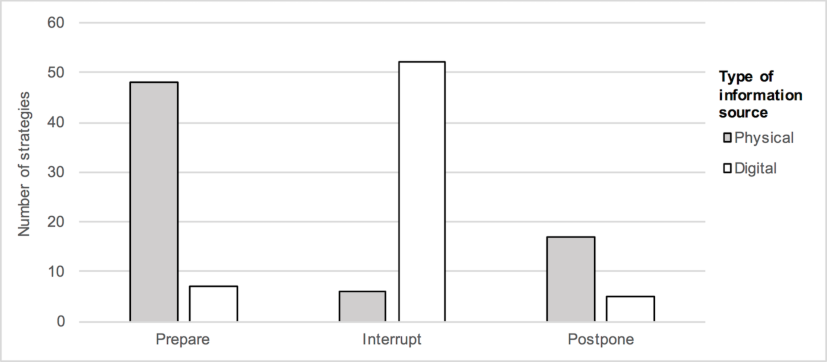
\includegraphics[scale=0.8]{images/ch12/ch12_graph.pdf}
\caption[Study 2 bar chart of interruption strategies]{Bar chart showing the number of strategies grouped in each high-level category for physical and digital information sources. The most common strategy to collect information from physical sources was to prepare information before starting a data entry task. The most common strategy to collect information from digital sources was to interrupt and switch to the source during a data entry task.}
\label{fig:ch12_graph}
\end{figure}

Table \ref{tbl:ch12_Table2} provides an overview of all strategies identified in the study \footnote{The data is available to download as a csv file at \url{https://osf.io/u2hy9/}} . The three columns of the table indicate the high-level categories. Each column is filled with examples of observed behaviour that fall under this high-level category, and numbers in parentheses indicate for which participants this behaviour was observed. These examples are further split into rows, to indicate for which particular information source this behaviour was observed. For example, in the top row it can be seen that participants P1-P9 Prepared (column) collecting a Paper claim form (row) by Placing it on their desk (top-left cell). Each row indicates a different information source: the top seven rows are Physical sources, and the bottom eight rows are Digital sources. I next provide more detailed examples of some of the strategies, first for physical sources and then for digital sources.

\begin{table}
\centering
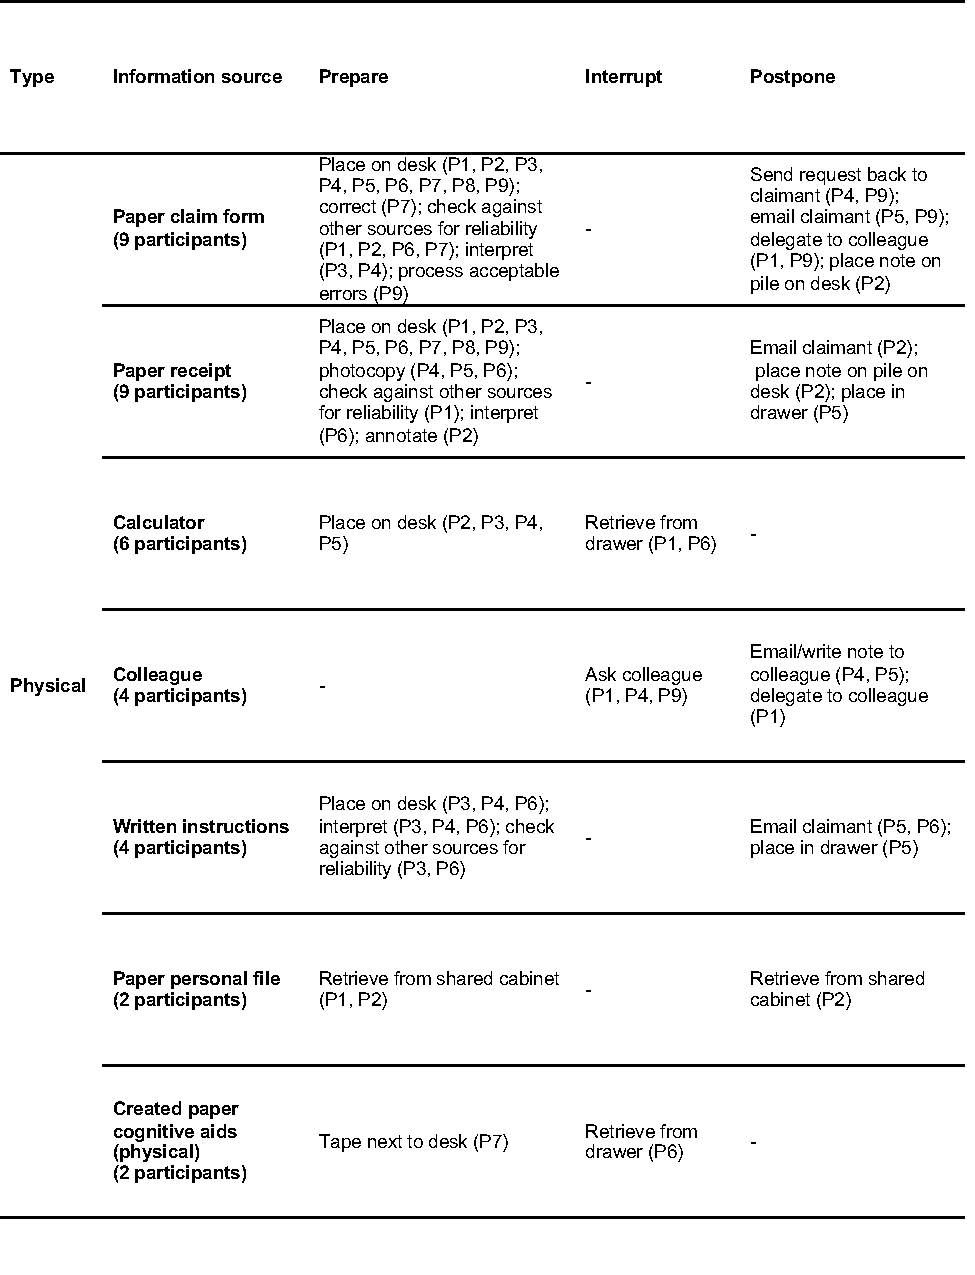
\includegraphics[scale=0.8]{images/ch12/ch12_TablePhys.pdf}
\end{table}
\begin{table}
\centering
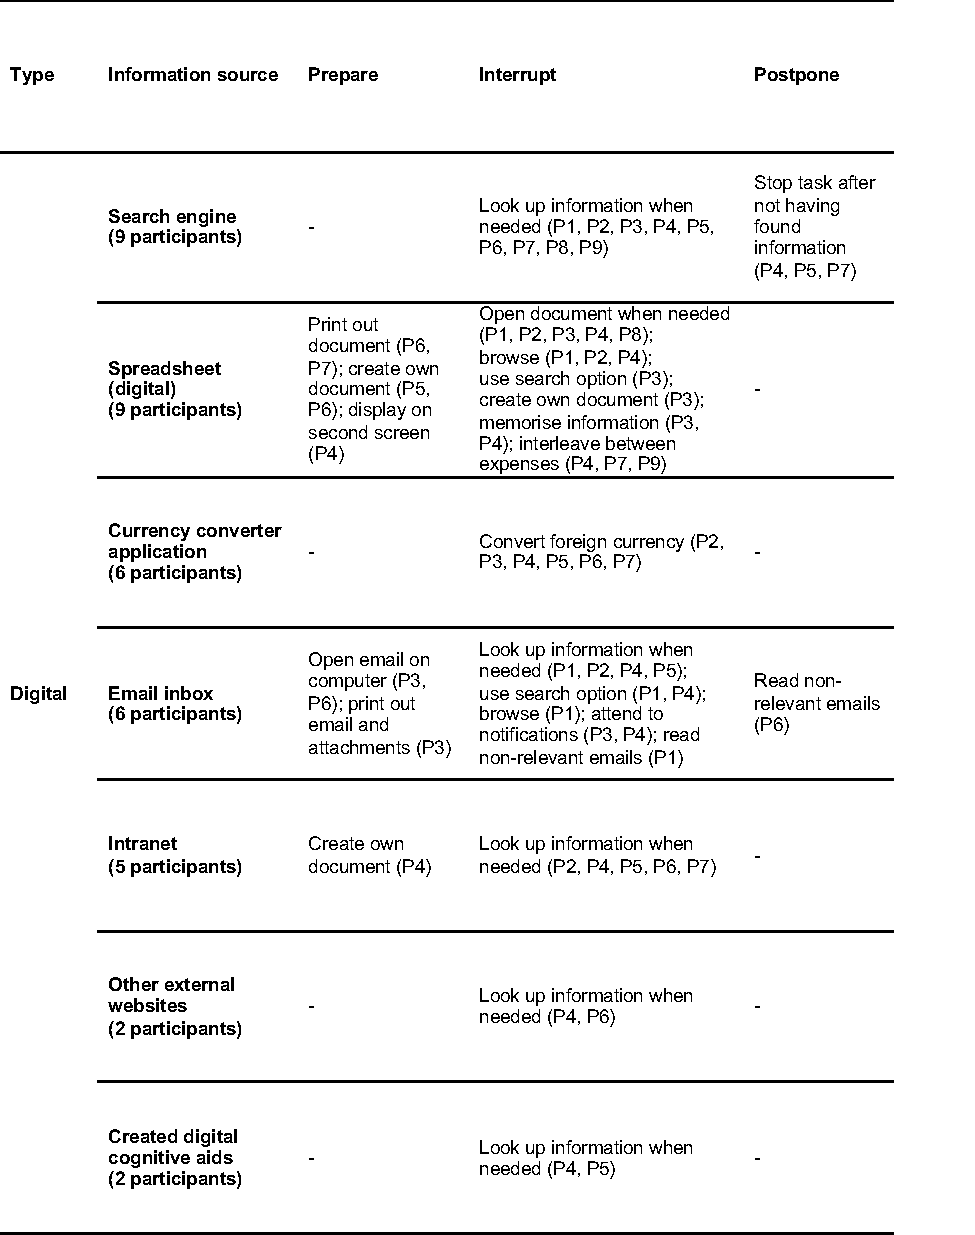
\includegraphics[scale=0.8]{images/ch12/ch12_TableDig.pdf}
\caption[Study 2 overview of observed inquiry strategies]{Overview of observed strategies to collect information. The columns indicate the three high-level categories Prepare, Interrupt and Postpone. Each column is filled with examples of observed behaviour that was categorised under this high-level category. Numbers in parentheses indicate for which participants this behaviour was observed. The rows indicate for which particular information source this behaviour was observed.}
\label{tbl:ch12_Table2}
\end{table}

\subsubsection{Paper information sources}
As in Study \hyperref[st:Study1]{1}, all participants were aware of the disruptiveness of interruptions, and the importance to focus on their data entry work: \textit{'Expenses claims, (…) they do require high detail to attention. So I like to make sure that's done before I do anything else.'} (P3 - interview). As a result, they avoided switching to unrelated tasks, and participants prepared most paper information sources before starting data entry work. As can be seen in the Prepare column of Table \ref{tbl:ch12_Table2}, several participants prepared sources such as claim forms, receipts, calculators and written instructions by placing them on their desk (P1-P9), personal files were retrieved from cabinets and drawers (P1, P2), or paper sheets were already taped on walls (P7). Participants inspected these sources, and sometimes retrieved additional information sources to check the reliability, \textit{'especially with foreign receipts, you don't really know (…) what they are.'} (P6). 

A common observation was that people often discovered that they needed additional information partway through working on a data entry task. If information was nearby, for example, if it was placed in a drawer (P6) or if it could be easily handed over by a colleague (P1, P4, P9), participants interrupted their data entry task and retrieved it straight away. 

If colleagues were not available and the information was situated further away, participants postponed looking for the information, and tried to complete other parts of the main task first. In some cases, it was not possible to progress with the task until the required information had been found. This often stopped the task altogether, and people switched to working on a different task instead. As shown in the Postpone column of Table \ref{tbl:ch12_Table2}, strategies to postpone collecting information included sending the claim request back to the claimant (P4, P9), sending an email to the claimant (P2), and writing a note to a colleague who could provide the information (P4, P5). For example, \textit{'I'm going to put this to one side. And come back to it. (…) What I do is just make a post-it note [writes post-it note], and just put it here [places it on a pile in left-hand corner of desk, and goes to new claim].'} (P2, think-aloud). 

\subsubsection{Digital information sources}
Participants tried to prepare some digital information sources beforehand as well, as illustrated at the bottom of the Prepare column of Table \ref{tbl:ch12_Table2}. For example, participants prepared spreadsheets by printing them out (P6, P7), displaying them on a second screen (P4), and opened a relevant email on their computer (P3, P6) in advance of starting a data entry task. 

As before, people often discovered that they needed additional information partway through working on a data entry task. However, when additional information was needed from a digital information source, rather than postpone looking it up, participants were far more likely to interrupt the task and retrieve it immediately. This can be seen by looking at the bottom rows of Table \ref{tbl:ch12_Table2}  and comparing the Interrupt and the Postpone column: most of the strategies for digital sources are grouped under the Interrupt column, while the Postpone column is mostly empty.  

Participants explained they tried to retrieve digital information immediately because they assumed that digital sources were easy to access and retrieving these involved little time away from the task. Interruptions to look up digital information could however take far longer than intended, as illustrated by the following quote from P4: \textit{'I go and make sure I’ve got the codes and stuff, ready to go. (…) I get halfway through and it goes, Oh, I don’t know what that is. And I have to look it up. Then I’ll get logged out, because it will take me longer than 5 minutes to do so.'} (P4, think-aloud). Three main underlying reasons for these unexpected time costs emerged from observations, and were supplemented by participants discussing past incidents. First, participants were observed going in and out of several documents to find what they were looking for (P1-P9), and sometimes could not find what they were looking for at all (P2, P4-P7). 

Second, participants had to search through large documents with irrelevant information (e.g. spreadsheet tables with 1,000 rows and 20 columns). For example, for each expense claim, a project code had to be entered to specify for which research project the expense was made. Participants had to find this code from a large spreadsheet that contained all codes used within the organisation. During observations, participants used the search option, but also regularly did not know what specific terms to look for, and ended up scanning through the document (P2, P4, P5, P8). 

Third, irrelevant information provided potential distractions and participants were observed being diverted, for instance when they had to find information in email. Email was used by participants both as a communication tool and information source. In its role as communication tool, participants tried to ignore it during data entry work, as it was considered distracting (P1, P2, P4-P6). However, they often needed to access it to find information relevant to their work. During the think-aloud part, P1 tried to find a relevant email and opened several emails to see if it had the information he was looking for. After opening one email, he quickly knew it was not relevant but continued to read it anyway, as it reminded him of something else he had to do later on the day.

These digital interruptions had negative consequences. First, the data entry system logged out after a period of inactive use, which forced participants to restart the task from the beginning: \textit{'You’d sit down to do something, and someone (…) or something distracts you, and by the time you go back, the system’s frozen and locked you out.'} (P4 - interview). Five participants reported they had experienced these logouts in the past (P4-P8), and in most cases their information was lost. Participants said the added cost of logouts kept them focused on the data entry task, and they were less likely to attend to external interruptions or switch to other, unrelated tasks. Observations however showed that each participant did interrupt their data entry and switched computer windows to look up digital information, without saving their data. Two participants were observed being logged out during the sessions (P6, P8). It was not clear to participants how long the system would wait before logging them out, or how long it would take to look up information, making it difficult to plan for these logouts: \textit{'It doesn’t time out, that’s why I call it a crash out. We tend to lose various amounts of information.'} (P8, think-aloud). 

A second negative consequence was that participants switched back to the wrong window, or entered the wrong information: \textit{'If you, by mistake, left that menu, and went into another linking menu that comes up with somebody else’s payroll number, you would never know that you’re inputting somebody else’s calculation into another record. You have to be so careful.'} (P9, think-aloud).

All window switches during data entry work happened on the same screen, even though most participants had access to two screens (P3-P9). Digital information was only displayed on a second screen if it was prepared beforehand and needed for a longer period of time: \textit{'If it was a credit card claim, (…), I would have the list of credit card expenditure on one screen, and then the claim on the other. But then I’d also have another tab where I can look up codes.'} (P4, think-aloud).

\subsection{Discussion}
The aim of this study was to investigate how people self-interrupt to access information sources for data entry work. Based on previous literature, it was expected that participants made fewer interruptions to information sources if these were harder to access. What was found however, is that participants were often unaware of how hard sources were to access, making it difficult to adapt their strategies. The results show that while task-unrelated interruptions are avoided, and people try to organise their data entry work so they can complete it uninterrupted, they regularly self-interrupt during the task to switch to digital information. They motivated this behaviour by saying they expected these switches to be short, but observations revealed that interruptions often took far longer than people intended, which suggests there is an unawareness of time spent on interruptions. In the next sections, I first discuss possible reasons for people's behaviour, and then discuss what the implications are for interruption management tools. 

%The aim of this study was to investigate how people self-interrupt data entry work to access task information. 

\subsubsection{Paper versus digital interruptions}
The first finding is that participants either carefully prepared paper information sources before starting a task or postponed retrieving it, but did interrupt themselves regularly during the task to switch to other computer windows and find additional digital information. One possible reason for this difference in behaviour is that these switches were not experienced as ‘interruptions’ from the activity, but rather just another part of the same activity. Participants stayed on the same monitor screen when switching windows, and explained they only used a second screen for different tasks. Though participants were observed switching between computer windows to find task information, interviews revealed that they do deliberately try to minimise interruptions to unrelated tasks as data entry work requires focused attention. While this may at first seem like a contradictory finding, it is important because it provides a nuanced understanding of how people think about inquiries. 

Window switching behaviour is consistent with previous research that has shown people switch between application windows when working on a computer every few minutes \citep{Gonzalez2004}. This study extends these findings by making a distinction between the types of windows people switch to. The findings suggest that even when people in this context are fairly good at reducing switches to irrelevant windows, they switch immediately to windows needed to locate information for the current task. 

\subsubsection{Time spent on an interruption}
Another possible reason for the different treatment of paper and digital sources is the time involved in retrieving them. Participants predominantly prepared or postponed physical sources, but some instances were observed where they interrupted their work to locate information necessary to complete the task. In these cases, the information was nearby in the physical environment and retrieved rather quickly. The findings suggest that people's decisions regarding whether or not to self-interrupt a task are influenced by the expected time involved in locating the information.

\subsubsection{Distracted by other information}
As described above, digital interruptions often took far longer to find than intended, as people had to spend effort finding what they needed and were distracted by other, task-irrelevant, information. A likely reason for this outcome was that people needed to access digital sources which are likely to be distracting, such as email. Arguably, participants were largely unaware of the time spent on these digital interruptions, as they adopted deferral strategies for non-digital interruptions when they perceived that they would take excessive amounts of time. This finding is important as it suggests that, even if an interruption is motivated by the goal to locate specific information and then return to the task, people can still get distracted by surrounding information. These distractions may make it difficult for people to be aware of the time that they actually spend on these interruptions – as a result, it is difficult for people to manage them effectively.

The tendency to attend to irrelevant information is similar to so-called chains of diversion, where the user diverts from the current task and forgets the original objective \citep{Hanrahan2015, Iqbal2007}. Previous work has explored tools that aim to prevent diversions during a task, for example by enabling users to group windows needed for the same task \citep{Smith2003} and disable switches to distracting sources \citep{Kim2017}. This study illustrates that these types of interventions may not be appropriate in situations where people do not know they need certain sources until they have started the task, and often need to access the sources they find distracting for work.

The study provides further insight in interruptions at the workplace and how task-related interruptions, presumed to be quick and easy, can end up being time-consuming and disruptive to work. This means we not only need to consider blocking interruptions that may be distracting from work, but also what support people can be given to control interruptions which are needed for, and considered part of, the task they want to focus on.

\subsubsection{Implications for interruption management tools}
The results provide useful initial insights for interruption management tools in the workplace, as they demonstrate that current interruption management tools can provide insufficient support to manage inquiries. First, whilst there are many tools that aim to block interruptions, (\citet{Lyngs2018} suggests that about 40\% of the 112 tools he reviewed in 2018 had this functionality), workers might benefit from adopting tools that do not block interruptions, but instead support deferral of self-interruptions until a more convenient moment in the task. For example, upon switching windows, users may be presented with a message discouraging them to switch immediately and an option to set a reminder to collect the required information later. This approach fits with the model proposed by \citet{Lyngs2018}, which uses the underlying cognitive mechanisms of self-regulation to frame self-regulation difficulties in ICT use. From the perspective of the model, difficulties occur because at the time of action, people's usage goals are either not strongly represented in working memory, or the value of meeting these goals is too low to control behaviour. By making people more aware of the value of deferring interruptions, or rather the harm of not deferring them, they may be more able to self-regulate their interruptions. 

Second, providing people with information about the length of their interruptions may help them self-regulate their interruptions better. One of the self-regulatory guidelines in Lyngs' model is to inform users about their behaviour. When applying this to the setting studied in this study, time information may in particular be appropriate, as participants in the study did already effectively manage some interruptions, when they presumed them to be time-consuming: they addressed them before starting a task or postponed them until later. People may be made more aware of time if they are given timed reminders to return to their task, or explicit feedback about the length of their self-interruptions. Reducing the length of interruptions can be very beneficial for data entry work, as the longer people interrupt, the more disruptive it is to their main task \citep{Altmann2017}.

Finally, though prior studies have shown that two screens can improve task immersion \citep{Bi2009}, in this study a second screen was largely unused for data entry work. In this case, an extra screen can have the contradicting effect of being distracting from work, if it is filled with task-irrelevant information. This finding highlights that the beneficial effect of multiple screens on productivity depends on the type of work: it loses its benefit if a task requires switching between various different documents, rather than one large document which can be displayed on one screen.

\begin{comment}
\subsubsection{Limitations}
%The office setting studied here allowed for video recordings and observations. The presence of an observer may have influenced people's behaviour, and people may self-interrupt more often or for longer with no observer present. However, due to the sensitive nature of financial data, it was not possible to install logging software on participants' computers and all observational data reported here is qualitative. It would be useful to conduct future studies at other office settings that will allow for additional quantitative data gathering techniques. 
This study highlights how different information sources can elicit different self-interruption strategies. Other possible factors contributing to people's strategies are user expertise and the type of role. In the studies reported in this chapter, job roles ranged amongst participants, but I did not observe any clear differences in strategy between junior and senior employees. This could however also be because junior employees were taught to do their work by their senior colleagues. Future studies are needed to get further insight to what extent job roles contribute to specific strategies.

Lastly, the study was conducted in a particular type of workplace. Although participants were in a range of job roles, they all worked at a financial administration office of a university, and care should be taken when generalising the results. For example, workers in a closed or home office may have fewer external interruptions by colleagues, and self-interrupt differently. I expect the results to apply to other office environments involving the use of paper and digital information.

\subsection{Conclusion}
Prior research has shown that work interruptions can have negative consequences on productivity and stress \citep{Mark2008}. This study contributes to this body of work by focusing on a specific type of interruption motivated by the need to access task information, and how these interruptions are managed differently for paper and digital information. A key insight from the study is that people regularly interrupt themselves to fetch digital information sources as and when they are needed to support a task. This is problematic and disruptive to the task, especially if digital information ends up being difficult to find and users get distracted while looking for it. In contrast, participants prepare physical information sources either before starting work or postpone to access it later. I hypothesise that the reason people work differently with these artefacts is because computer window switches are seen as part of the same activity, because of preconceptions about ease of access, and because of lack of awareness of time spent on digital interruptions. 
\end{comment}

\section{Summary of Chapter 3}
The aim of this chapter was to get a better understanding of how people manage inquiries for data entry work in an office setting. Study \hyperref[st:Study1]{1} showed that people try to avoid task-irrelevant interruptions, but have to make inquiries as part of data entry tasks, and a critical component of data entry work is not just entering the data, but also retrieving data from multiple sources distributed in the environment. Study \hyperref[st:Study2]{2} showed that people try to prepare and collect most physical information before starting a data entry task. However, computer window switches during the task were commonly observed as workers often realised during the task that they needed additional information. Digital interruptions often took far longer than people intended, and this had a negative impact on work: software logged users out because of inactivity and they made errors on resumption, entering information in the wrong fields, or entering information incorrectly. These findings suggest that people do not always know how to effectively manage digital self-interruptions that are seen as part of the same activity. 

Based on these findings, I make the hypothesis that presumed time costs involved to collect information play an important part in how people address self-interruptions, and that workers are unaware of the time they actually spend on digital interruptions. However, all findings reported in this chapter are qualitative, and are insufficient to make any concluding claims on the effect of time costs on interruption strategies. The use of interviews and observations were suitable to get a better understanding of how data entry work is situated in an office setting and people's self-interruption strategies during this work, but the extent to which these strategies were influenced by the observed time costs associated with inquiries is unclear. Therefore, the next chapter reports three lab experiments to study the effect of time costs on people's interruption behaviour in a controlled setting, and to measure the effect of these strategies on data entry performance.

